\chapter{Design}

\section{Overall System Design}

\subsection{Short description of the main parts of the system}
\textbf{Gas, Electricity and Water metering system}
\begin{itemize}
\item{User Interface}
\item{Graphs and Charts}
\item{Database control}
\end{itemize}
User Interface:
\begin{itemize}
\item{The user will be presented with an interface which has two text boxes for the username and password and a button to proceed once they have entered their login details. These details will be unique and should only be known by the user they pertain to.}
\item{Once logged in to the system, the user will be presented with a new interface in which they can load a database and access the different functionalities of the system such as inputting readings from the meters into the system to be stored in the database, viewing calculated averages and future prices and viewing consumption rates for the current month and any previous months in different formats and graphs/charts.}
\item{The user will be able to navigate the different tabs of the interface via keyboard input or through tab buttons on a toolbar on the system}
\end{itemize}

Graphs and Charts:
\begin{itemize}
\item{There will be several Graphs and charts on the system such as Pie Charts, Bar Charts, Line Graphs, Scatter Diagrams, tables etc. This is beneficial because it means that the user has a range of visual representations to choose from and can therefore choose the one they like the most or can understand and interpret the easiest. Each type of chart will have their own individual tab on the main interface.}
\item{There will be 3 of each type of chart/graph for Gas, Electricity and Water Consumption, with each set of charts/graphs on a tab.}
\end{itemize}

Database control:
\begin{itemize}
\item{On the menu bar and toolbar there will be options to open to close a database, format the database  or create a new one along with options to add or remove items from the database each with icons to represent them for ease of access}
\item{In addition to these buttons, there will be added functionality for keyboard shortcuts to make using the system as quick as possible}
\item{If the user chooses to add data then they will be taken to an interface which asks what table the data is for and if relevant, which consumption type it refers to and then the system will take the user to a new interface in which they can input the data they wish to add and submit it to the database.}
\item{If the user chooses to remove data from the database, they will be taken to a similar interface to the one for the input interface and will be asked to specify what this data pertains to and then provide a date and consumption type if relevent.}
\item{If the user chooses to format the database then they will be taken to a new interface which asks them if they are sure that they want to format the database and will have two buttons for confirmation}
\item{If the user chooses to create a new database, they will be taken to another interface where they will be prompted to input a name for the new database and the interface will also contain a button which when pressed prompts the user to find the location on their computer to store the new database}
\end{itemize}

\subsection{System flowcharts showing an overview of the complete system}

\section{User Interface Designs}
\begin{figure}[H]
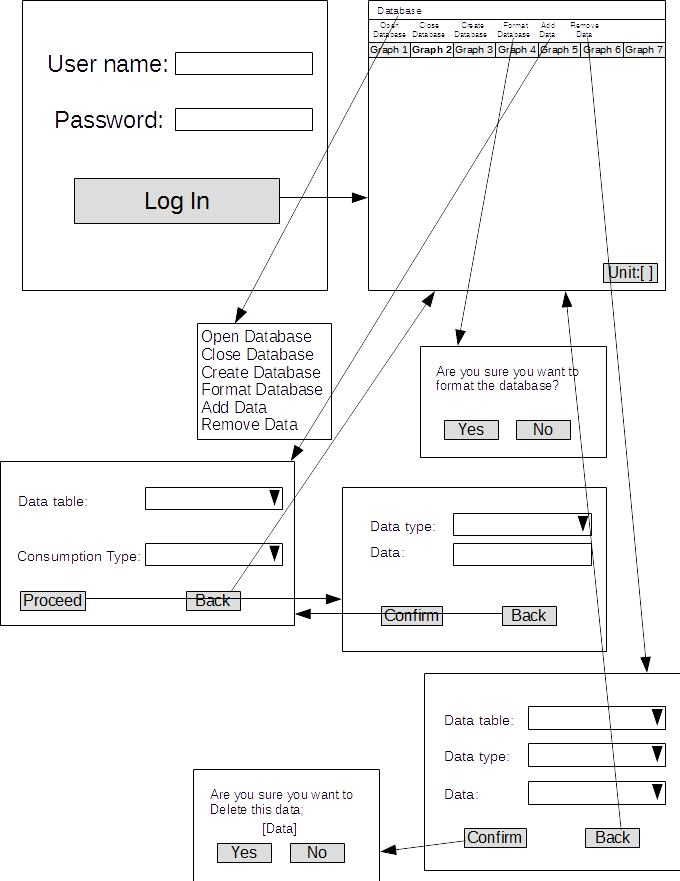
\includegraphics{./design/User Interface Design.png}
\caption{User Interface Design}
\end{figure}

\section{Hardware Specification}
The system will need to run on a laptop with a 1366x768 resolution screen with a 16:9  aspect ratio and running Windows 8. This is significant because it means I need to make sure the program will fit to this screen. A mouse will be srequired to navigate the program and select any inputs from drop down menus and a keyboard will be required to input data into text boxes on the program. The database for the program will be stored on a 1tb internal hard drive.
\section{Program Structure}

\subsection{Top-down design structure charts}

\subsection{Algorithms in pseudo-code for each data transformation process}

\subsection{Object Diagrams}

\subsection{Class Definitions}

\section{Prototyping}

\section{Definition of Data Requirements}

\subsection{Identification of all data input items}

\subsection{Identification of all data output items}

\subsection{Explanation of how data output items are generated}

\subsection{Data Dictionary}

\subsection{Identification of appropriate storage media}

\section{Database Design}

\subsection{Normalisation}

\subsubsection{ER Diagrams}
\begin{figure}[H]
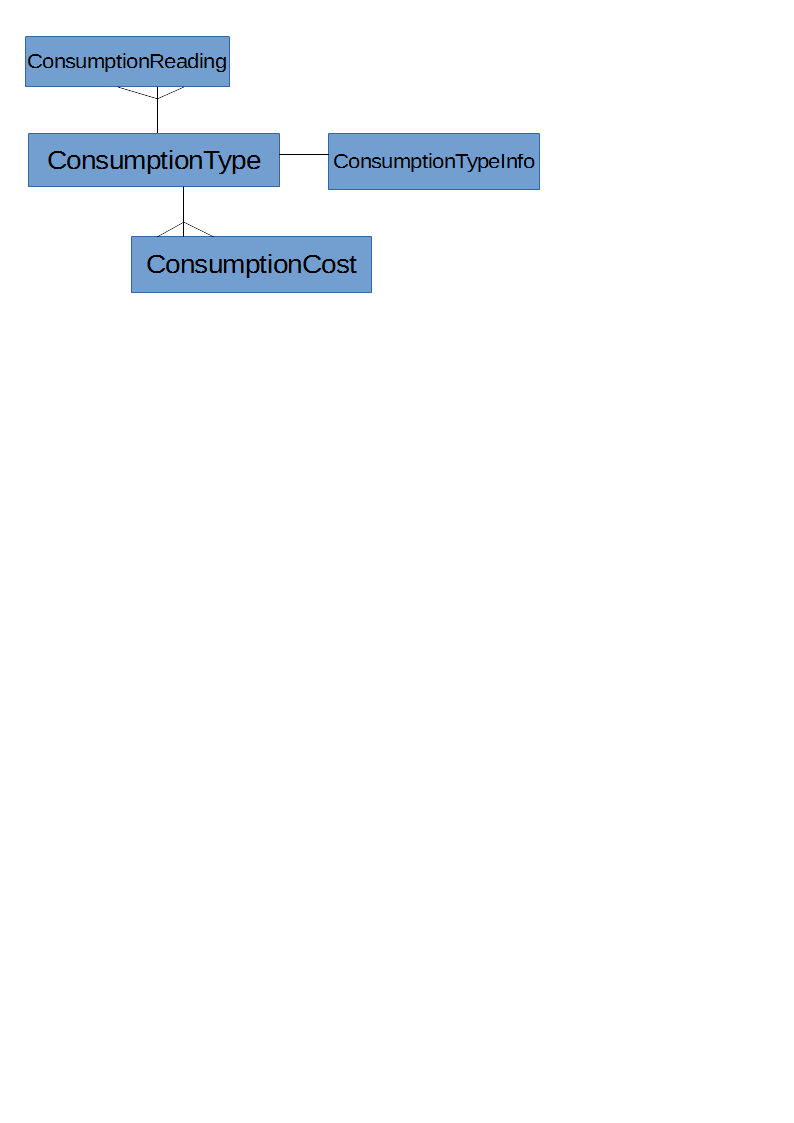
\includegraphics{./design/ER Diagrams.png}
\caption{ER Diagram}
\end{figure}

\subsubsection{Entity Descriptions}
Type(\underline{TypeID}, ConsumptionType,ConsumptionTypeDescription) \\
Reading(\underline{ReadingID},ConsumptionReading,ReadingDate,\emph{ConsumptionType}) \\
UserReading(\underline{UserReadingID},\emph{UserID},\emph{ReadingID}) \\
User(\underline{UserID},FirstName,LastName,UserPassword) \\
Cost(\underline{CostID},CostPerUnit,CostStartDate) \\
TypeCost(\underline{TypeCostID},\emph{CostID},\emph{ConsumptionType})\\

\subsubsection{1NF to 3NF}
\begin{center}
	\begin{tabular}{|p{5cm}|}
		\hline
		\textbf{UNF} \\ \hline
		UserID \\ \hline
		FirstName \\ \hline
		LastName \\ \hline
		UserPassword \\ \hline
		ReadingID \\ \hline
		ConsumptionReading \\ \hline
		ReadingDate \\ \hline
		ConsumptionType \\ \hline
		ConsumptionTypeDescription \\ \hline
		CostID \\ \hline
		CostPerUnit \\ \hline
		CostStartDate \\ \hline
	\end{tabular}
	
	\begin{tabular}{|p{5cm}|p{3.5cm}|}
		\hline
		\textbf{1NF} &  \\ \hline
		\textbf{Repeating} & \textbf{Non-repeating} \\ \hline
		\underline{ReadingID} \underline{UserID} & \underline{UserID} \\ \hline
		ReadingDate & FirstName \\ \hline
		ConsumptionReading & LastName\\ \hline
		ConsumptionType & UserPassword \\ \hline
		ConsumptionTypeDescription & \\ \hline
		CostID & \\ \hline
		CostPerUnit & \\ \hline
		CostStartDate & \\ \hline
	\end{tabular}

	\begin{tabular}{|p{5cm}|p{5cm}|p{3cm}|}
		\hline
		& \textbf{2NF} & \\ \hline
		\underline{ReadingID} \underline{UserID} & \underline{ReadingID} & \underline{UserID} \\ \hline
		ConsumptionReading & ConsumptionType & FirstName \\ \hline
		ReadingDate & ConsumptionTypeDescription & LastName \\ \hline
		 & CostID & UserPassword \\ \hline
		 & CostPerUnit & \\ \hline
		 & CostStartDate & \\ \hline
	\end{tabular}

	\begin{tabular}{|p{5cm}|p{4cm}|p{3.5cm}|}
		\hline
		 & \textbf{3NF} & \\ \hline
		\textbf{Type} & \textbf{Reading} & \textbf{UserReading} \\ \hline
		\underline{TypeID} & \underline{ReadingID} & \underline{UserReadingID} \\ \hline
		ConsumptionType & ConsumptionReading & \emph{ReadingID} \\ \hline
		ConsumptionTypeDescription & ReadingDate & \emph{UserID} \\ \hline
		 & \emph{TypeID} & \\ \hline
		 & & \\ \hline
		\textbf{User} & \textbf{cost} & \textbf{TypeCost} \\ \hline
		\underline{UserID} & \underline{CostID} & \underline{TypeCostID} \\ \hline
		FirstName & CostPerUnit & \emph{CostID} \\ \hline
		LastName & CostStartDate & \emph{TypeID} \\ \hline
		UserPassword & & \\ \hline
	\end{tabular}
\end{center}

\section{Security and Integrity of the System and Data}

\subsection{Security and Integrity of Data}

\subsection{System Security}
To make sure the system is secure I will be implementing several access restrictions on the system such as a username and password that the user will choose and  set and each time the system is used the user will be required to input the chosen username and password before they can gain access to the system. To keep the username and password secure I will also be encrypting them and making sure that they are only accessed when needed to compare what the user has provided for a username and password.
\section{Validation}

\section{Testing}

\begin{landscape}
\subsection{Outline Plan}

\begin{center}
    \begin{tabular}{|p{2cm}|p{5cm}|p{5cm}|p{4cm}|}
        \hline
        \textbf{Test Series} & \textbf{Purpose of Test Series} & \textbf{Testing Strategy} & \textbf{Strategy Rationale}\\ \hline
        Example & Example & Example & Example \\ \hline
    \end{tabular}
\end{center}

\subsection{Detailed Plan}

\begin{center}
    \begin{longtable}{|p{1.5cm}|p{2.5cm}|p{2.5cm}|p{2cm}|p{2cm}|p{2cm}|p{2cm}|p{2cm}|}
        \hline
        \textbf{Test Series} & \textbf{Purpose of Test} & \textbf{Test Description} & \textbf{Test Data} & \textbf{Test Data Type (Normal/ Erroneous/ Boundary)} & \textbf{Expected Result} & \textbf{Actual Result} & \textbf{Evidence}\\ \hline
        Example & Example & Example & Example & Example & Example & Example & Example \\ \hline
    \end{longtable}
\end{center}
\end{landscape}
